\documentclass[../../thesis.tex]{subfiles}
\begin{document}

\chapter{Results and Analysis}
\label{sec:RESULTS}
\pcstart{ch4}{10}

\chaptertitleblock
  {\QuoteChIV}
  {\AttribChIV}
  {This chapter presents the results of the data analysis and their interpretation. After the data sample (\cref{sec:RESULTS_DATA_SAMPLE}), the event selection (\cref{sec:RESULTS_EVENT_SELECTION}), the background estimation (\cref{sec:RESULTS_BACKGROUND_ESTIMATION}) and the systematic uncertainties (\cref{sec:RESULTS_SYSTEMATIC_UNCERTAINTIES}), \cref{sec:RESULTS_RESULTS,sec:RESULTS_STATISTICAL_SIGNIFICANCE} give the measurement and its significance, and \cref{sec:RESULTS_COMPARISON_WITH_PREVIOUS_RESULTS,sec:RESULTS_INTERPRETATION} compare and interpret it.}

\clearpage
\section{Data Sample}
\label{sec:RESULTS_DATA_SAMPLE}
\pcstart{s41}{2}

The analysis is based on proton-proton collision data collected during [time period], corresponding to an integrated luminosity of [value] fb$^{-1}$ at $\sqrt{s} = $ [value] TeV.

\pcend{s41}

\section{Event Selection}
\label{sec:RESULTS_EVENT_SELECTION}
\pcstart{s42}{2}

\subsection{Selection Criteria}
\label{sec:RESULTS_EVENT_SELECTION_SELECTION_CRITERIA}

Events are required to satisfy the following criteria:
\begin{itemize}
  \item Pass trigger requirements
  \item Contain [specific particles/objects]
  \item Satisfy kinematic cuts: $p_T > $ [value] GeV, $|\eta| < $ [value]
\end{itemize}

\subsection{Selection Efficiency}
\label{sec:RESULTS_EVENT_SELECTION_SELECTION_EFFICIENCY}

The overall selection efficiency is \resExampleSignalEfficiency, the product of the trigger, reconstruction and selection efficiencies:
\begin{equation}
  \epsilon_{\mathrm{total}} = \epsilon_{\mathrm{trigger}} \times \epsilon_{\mathrm{reco}} \times \epsilon_{\mathrm{selection}}.
  \label{eq:efficiency}
\end{equation}

\pcend{s42}

\section{Background Estimation}
\label{sec:RESULTS_BACKGROUND_ESTIMATION}
\pcstart{s43}{2}

\subsection{Major Background Processes}
\label{sec:RESULTS_BACKGROUND_ESTIMATION_MAJOR_BACKGROUND_PROCESSES}

The main background contributions come from:
\begin{itemize}
  \item [Background process 1]
  \item [Background process 2]
  \item [Background process 3]
\end{itemize}

\subsection{Background Normalization}
\label{sec:RESULTS_BACKGROUND_ESTIMATION_BACKGROUND_NORMALIZATION}

Background rates are normalized using control regions in data.

\pcend{s43}

\section{Systematic Uncertainties}
\label{sec:RESULTS_SYSTEMATIC_UNCERTAINTIES}
\pcstart{s44}{2}

\subsection{Experimental Uncertainties}
\label{sec:RESULTS_SYSTEMATIC_UNCERTAINTIES_EXPERIMENTAL_UNCERTAINTIES}

Major sources of experimental uncertainty include:
\begin{itemize}
  \item Luminosity: [value]\%
  \item Trigger efficiency: [value]\%
  \item Reconstruction efficiency: [value]\%
  \item Energy scale: [value]\%
  \item Energy resolution: [value]\%
\end{itemize}

\subsection{Theoretical Uncertainties}
\label{sec:RESULTS_SYSTEMATIC_UNCERTAINTIES_THEORETICAL_UNCERTAINTIES}

Theoretical uncertainties arise from:
\begin{itemize}
  \item PDF uncertainties
  \item Scale variations
  \item Higher-order corrections
\end{itemize}

\pcend{s44}

\section{Results}
\label{sec:RESULTS_RESULTS}
\pcstart{s45}{2}

\subsection{Observed Distributions}
\label{sec:RESULTS_RESULTS_OBSERVED_DISTRIBUTIONS}

\Cref{fig:main-result} shows the [key observable] distribution.

\begin{figure}[htbp]
  \centering
  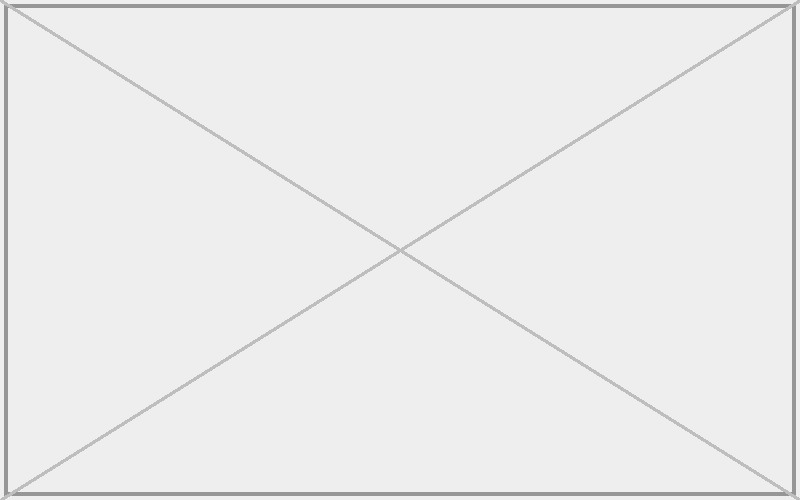
\includegraphics[width=0.7\textwidth]{figures/placeholder.png}
  \caption{Distribution of [observable] in data compared with the \gls{mc} prediction. [State the key takeaway.] \adaptedfrom{higgs-discovery}}
  \label{fig:main-result}
\end{figure}

\subsection{Signal Extraction}
\label{sec:RESULTS_RESULTS_SIGNAL_EXTRACTION}

The signal yield is extracted using [method]:
\begin{equation}
  N_{signal} = [value] \pm [stat] \pm [syst]
  \label{eq:signal-yield}
\end{equation}

\subsection{Measurement}
\label{sec:RESULTS_RESULTS_MEASUREMENT}

The measured [cross section/branching ratio/etc.] is:
\begin{equation}
  \sigma \times BR = [value] \pm [stat] \pm [syst] \text{ pb}
  \label{eq:measurement}
\end{equation}

This result is consistent with the Standard Model prediction of [value] pb.

\pcend{s45}

\section{Statistical Significance}
\label{sec:RESULTS_STATISTICAL_SIGNIFICANCE}
\pcstart{s46}{2}

The statistical significance of the observation is \resExampleSignificance$\sigma$, indicating [level of evidence].

\pcend{s46}

\section{Comparison with Previous Results}
\label{sec:RESULTS_COMPARISON_WITH_PREVIOUS_RESULTS}
\pcstart{s47}{2}

Our result is compared with previous measurements:
\begin{itemize}
  \item Previous experiment A: [value] $\pm$ [uncertainty]
  \item Previous experiment B: [value] $\pm$ [uncertainty]
  \item This work: [value] $\pm$ [uncertainty]
\end{itemize}

\pcend{s47}

\section{Interpretation}
\label{sec:RESULTS_INTERPRETATION}
\pcstart{s48}{2}

The results [support/constrain/exclude] [theoretical models/parameter space]. Implications for [physical interpretation] are discussed.

\pcend{s48}


\pcend{ch4}
\end{document}
